\chapter[Metodologia]{Metodologia}

\section{Scrum}

O Scrum é uma metodologia Ágil criada por Jeff Sutherland junto com Ken Schwaber em uma época onde o principal método de desenvolvimento de Software era o Cascata, uma abordagem linear, pouco flexível, o Scrum veio como uma mudança radical e muito mais flexível de desenvolver Software, contando com Sprints, adaptação contínua e reuniões regulares.
As Sprints são ciclos de desenvolvimento breves, e no início de cada uma, acontece uma reunião de planejamento da Sprint, onde a equipe decide uma quantidade de trabalho que será possível realizar nas próximas duas semanas. \cite{shuterland2014}

Dada a natureza do trabalho e o tamanho da equipe, não utilizamos efetivamente todas as práticas do Scrum como Sprints e suas cerimônias, uma vez que atuamos majoritariamente na resolução de erros, defeitos e falhas, que naturalmente são tarefas difíceis de estimar. Implementar o Scrum adicionaria uma complexidade desnecessária a um projeto com objetivos tão claros e um time de desenvolvimento tão pequeno.

Ainda assim optamos por incorporar alguns elementos do Scrum, como a alta adaptabilidade e flexibilidade e também uma equipe de desenvolvimento auto gerenciável e multifuncional, composta pelos autores deste trabalho. Esta abordagem proporcionou flexibilidade e adaptabilidade ao longo deste trabalho, permitindo ajustes em caso de eventuais mudanças de planos ou adversidades, e também com que a equipe fosse suficiente em si mesma.

\section{Extreme Programming}
O Extreme Programming (XP) é uma metodologia ágil de desenvolvimento de software, segundo Kent Beck, esta metodologia tem como valores: comunicação, simplicidade, \textit{feedback}, coragem e respeito. As práticas do XP enfatizam a flexibilidade, comunicação do time, entregas contínuas e \textit{feedbacks} rápidos, para melhorar a produtividade da equipe e a qualidade do software. Esta metodologia tem como algumas de suas práticas a programação em par, desenvolvimento orientado a testes, integração contínua e pequenas entregas frequentes. \cite{kentbeck2014}

Com o objetivo de orientar o desenvolvimento do trabalho, incorporamos ao nosso fluxo de desenvolvimento duas práticas características do XP, a programação em par e a integração continua. A escolha dessas práticas específicas se deu devido às características do time e as necessidades encontradas no escopo do projeto. Por se tratar de um projeto desenvolvido por duas pessoas, a adoção da programação em par ocorreu de forma natural e proveitosa. Além disso, a integração de cada nova versão ao aplicativo publicado na Google Play Store e ao servidor hospedado na AWS, foi essencial para evitar a descoberta tardia de incompatibilidades entre versão publicada e ambiente local.

\subsection{Programação em par}
A programação em par é uma prática do XP em que dois desenvolvedores trabalham juntos em uma mesma máquina para escrever o código. Durante o desenvolvimento, ambos devem estar concentrados no código desenvolvido dando sugestões e compartilhando conhecimento. Durante o desenvolvimento em par existe dois papéis, o piloto e o copiloto. O piloto é quem escreve o código e copiloto é quem revisa o código em tempo real, os papeis não são fixos e podem ser trocados a qualquer momento.

Devido às características do projeto, a programação em par trouxe grandes benefícios. Por se tratar de um projeto realizado em dupla, a sua adoção se deu de forma natural. Ela foi fundamental principalmente no momento de encontrar soluções para falhas críticas que demandam a análise de vários possíveis cenários para encontrar a causa, possibilitando pensar em uma quantidade maior de cenários através de duas perspectivas diferentes.

\subsection{Integração contínua}
A integração contínua consiste na prática de disponibilizar o código desenvolvido na aplicação principal o mais rapidamente possível, evitando o acúmulo de grandes quantidades de novas funcionalidades, correções de defeitos e melhorias para serem incorporadas de uma só vez à aplicação. Essa prática oferece vantagens significativas, como a detecção precoce de erros e rápida integração.

A integração contínua foi essencial para o projeto, especialmente devido ao processo necessário para a publicação de um aplicativo na Google Play Store, que envolve análises que podem levar até sete dias. Com a integração contínua, foi possível obter \textit{feedbacks} mais rápidos a cada nova versão publicada, evitando surpresas que poderiam ocorrer caso todo o código desenvolvido fosse integrado apenas ao final do trabalho.

\section{Roadmap}
Um \textit{roadmap} é um diagrama que define passos necessários para alcançar um determinado resultado ao longo de um período. Serve como um guia visual para mostrar a direção e o progresso do trabalho.

A partir dos nossos objetivos foi elaborado um \textit{roadmap} como apresentado na Figura \ref{roadmap}. O \textit{roadmap} foi utilizado com uma ferramenta para auxiliar o desenvolvimento e a organização das tarefas, entretanto, naturalmente algumas tarefas foram feitas paralelamente, contrariando a linearidade proposta no \textit{roadmap}. Isso foi feito para não permitir que o \textit{roadmap}, que é um artefato para nosso auxilio, viesse a prejudicar a eficiência da equipe na realização das atividades.

\begin{figure}[h]
	\centering
	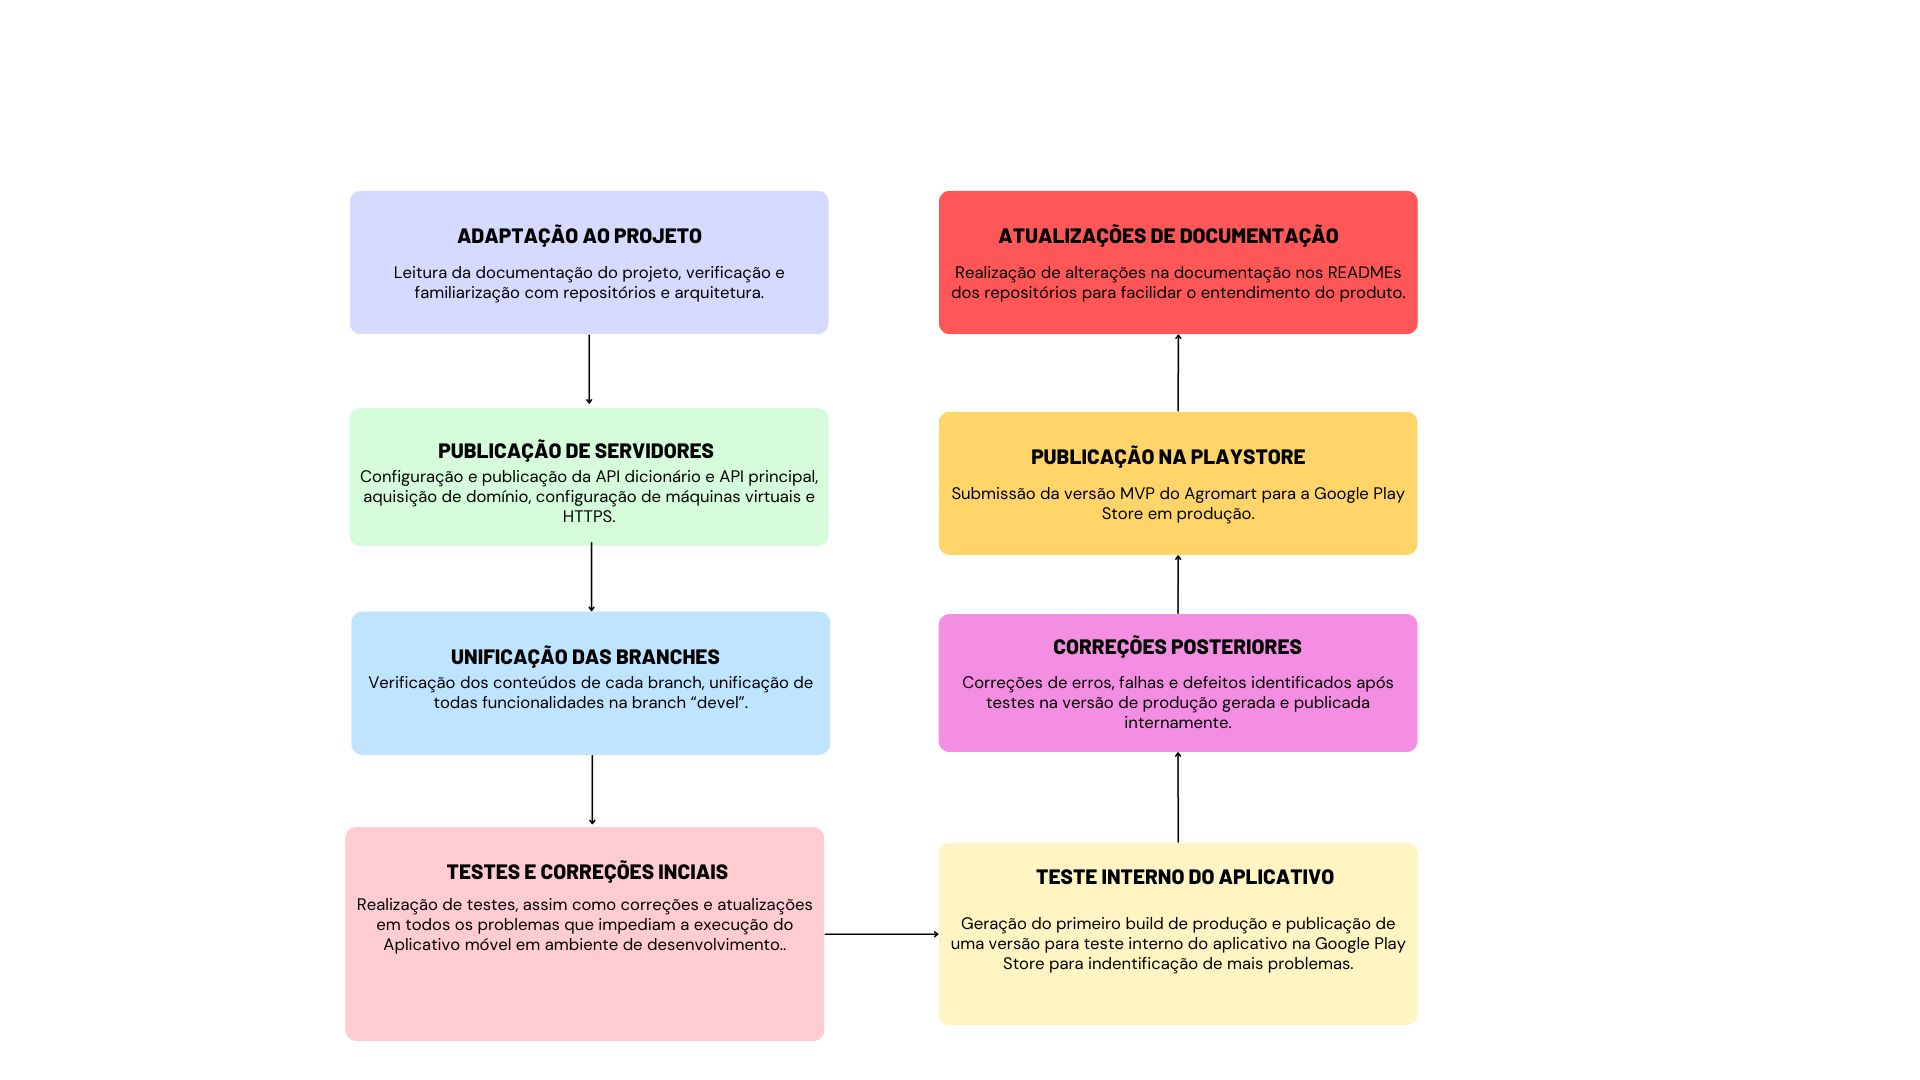
\includegraphics[keepaspectratio=true,scale=0.3]{figuras/roadmap2.png}
	\caption{\textit{Roadmap} proposto}
	\label{roadmap}
\end{figure}

A seguir, cada subseção apresenta uma breve descrição das atividades propostas no \textit{roadmap}.

\subsection{Adaptação ao projeto}
Essa atividade consiste na leitura da documentação do projeto e familiarização com repositórios, arquitetura e tecnologias empregadas.

\subsection{Publicação de servidores}
Se refere à configuração e publicação da API dicionário e API principal, aquisição de domínio e configuração de máquinas virtuais com certificado. Foi uma das atividades realizadas no início do trabalho para permitir maior produtividade na correção de erros, falhas e defeitos, já que os ambientes podiam ser acessados sem a necessidade de execução local.

\subsection{Unificação das \textit{branches}}
A atividade consiste na verificação dos conteúdos de cada \textit{branch}, unificação de todas funcionalidades na \textit{branch} “devel”. Essa atividade representa partida para o desenvolvimento.

\subsection{Testes e correções}
Realização de testes de caixa preta após a unificação das \textit{branches}, assim como correções e atualizações em todos os problemas que impediam a execução do aplicativo móvel em ambiente de desenvolvimento. Essa atividade foi realizada em paralelo com as atividades descritas a seguir, pois os defeitos eram sempre corrigidos a medida com que eram descobertos.

\subsection{Teste interno do aplicativo}
Geração da primeiro versão de produção e publicação de uma versão para teste interno do aplicativo na Google Play Store para identificação de problemas antes da publicação definitiva.

\subsection{Publicação na Play Store}
Consiste na submissão da versão MVP do Agromart para a Google Play Store em produção.

\subsection{Atualizações de documentação}
Essa é a ultima atividade proposta no \textit{roadmap}, que consiste na realização de alterações na documentação nos arquivos \texttt{README.md} dos repositórios para facilitar o entendimento do produto. 

\section{Versionamento de código}

\subsection{Git}
O Git \cite{git2024} é um sistema de controle de versão distribuído usado para gerenciar e rastrear alterações em projetos de software. Cada desenvolvedor mantém uma cópia completa do repositório, o que facilita o trabalho colaborativo de forma offline. Uma característica do Git muito importante no contexto deste trabalho é o conceito de \textit{branches}, que são ramos de desenvolvimento separados, desse modo, é possível desenvolver funcionalidades de forma isolada e, posteriormente, integrar essas mudanças ao projeto principal através de uma ação que chamamos de \textit{merge} ou mesclamento.

Nos dias de hoje o Git é uma ferramenta fundamental para o desenvolvimento de software, pois garante organização de versões e facilita o trabalho colaborativo  '. Ele pode ser integrado com diversas plataformas que hospedam código-fonte como o Github, GitLab, Bitbucket e Azure Repos. 

\subsection{GitHub}
O GitHub é uma plataforma que hospeda o código fonte de projetos que utilizam Git. Ele é usado para armazenar e facilitar o acesso à projetos de software que utilizam o Git para o seu versionamento \cite{github2024}. Além disso ele oferece recursos como \textit{pull requests}, que possibilita solicitar a junção de \textit{branches}, e revisão de código, em que é possível aprovar ou solicitar mudanças em uma \textit{pull request}. Ele é amplamente utilizada tanto em projetos \textit{open-source} quanto em ambientes corporativos, e é a plataforma onde o código fonte do Agromart é hospedado.

\subsection{GitFlow}

Após a unificação das \textit{branches} já existentes, foi feito o uso do GitFlow, que é uma política de organização de versionamento de código criado com o intuito de melhorar o fluxo das \textit{branches} nos repositórios. A Figura \ref{gitflow} apresenta a política de \textit{branches} de forma detalhada. O GitFlow já é o padrão do Agromart, porém como ficaram muitas \textit{branches} soltas sem serem devidamente fechadas, mostra que não foi utilizado corretamente em todos momentos, porém, neste trabalho, não foram deixadas \textit{branches} soltas, proporcionando um ambiente onde a prática do GitFlow se torna muito mais fácil e intuitiva.

\begin{figure}[h]
	\centering
	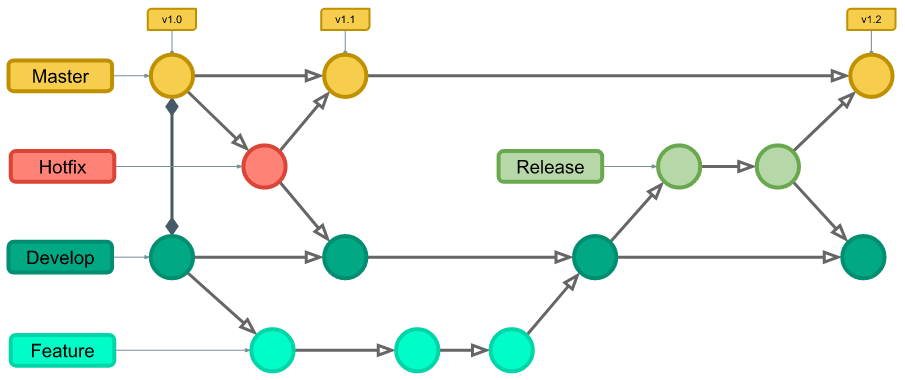
\includegraphics[keepaspectratio=true,scale=0.5]{figuras/gitflow.png}
	\caption{Representação gráfica do GitFlow}
    Fonte: \cite{alura2023}
	\label{gitflow}
\end{figure}


